\documentclass[letterpaper]{article} 			     	%articulo tamaño carta

\usepackage{booktabs} 								  	%Tablas bonitas de libro 
\usepackage[table,xcdraw]{xcolor} 					  	%tablas de latextable.com
\usepackage{anysize} 								  	%Definir margenes a gusto
\usepackage[english]{babel}				  				%Idioma						  
\usepackage[utf8]{inputenc} 						  		%Tildes y eñes
\usepackage{graphicx,epstopdf,pdfpages,float}		  	%Para poder insertar figuras, imagenes vectoriales, .pdf's y para fijar imagenes y tablas [H], resp.
\usepackage{latexsym,amsmath,amssymb,amsfonts,dsfont} 	%Caracteres propios de matematica, como el simbolo de los Reales
\usepackage{listings} 				                  	%Permite insertar codigos en C,MATLAB,ettc
\usepackage{color}									  	%Colour Fonts and other related features
\usepackage{multicol}[1999/05/25]					  	%Multiple Text Columns 	
\usepackage{subfigure}								  	%Subfigures
\usepackage{comment}

% Margenes: izquierda derecha arriba abajo
\marginsize{2 cm}{2 cm}{2 cm}{2 cm}  	

% Comandos definidos por usuario
\providecommand{\abs}[1]{\lvert#1\rvert} 	  % Valor absoluto
\providecommand{\norm}[1]{\lVert#1\rVert}	  % Norma
\newcommand{\HRule}{\rule{\linewidth}{0.5mm}} % Linea Horizontal Bonita
\newcommand{\red}{\textcolor{red}}
\newcommand{\white}{\textcolor{white}}

%Modifica encabezados de articulo (section, subsection, ettc)
\usepackage{titlesec}

\titleformat{\section}[block]
{\normalfont\sffamily}
{\thesection}{.5em}{\titlerule\\[.8ex]\bfseries}

\titleformat{\subsection}[block]
{\normalfont\sffamily}
{\thesubsection \bfseries}{.5em}{\bfseries}

\titleformat{\subsubsection}[block]
{\normalfont\sffamily}
{\thesubsubsection}{.5em}{\titlerule\\[.8ex]\bfseries}

% define indent size
\setlength\parindent{0cm}

\begin{document}

\textbf{Numerical Examples of the Surrogate Model for the Monodomain Equations with the Minimal Reaction Model}

\small{Felipe Galarce - PUCV}

\section{Mesh for the Spatial Discretization}

The mesh for the exact problem is composed by triangles of characteristic size 0.1 [mm], and is refined nearby the collagen inclusions, in order to correctly consider the mesoscale into the model. The refined elements have a characteristic size of 0.02 [mm]. On the other hand, the mesh used to solve the homogenized problem have a characteristic length of 0.5 [mm]. This difference is a consequence of the fact that the homogenized model does not need explicitily the mircoscale in the model, because the microscopic propiertes are considered in the effective macroscopic tensor. 

Note that the mesh size for the homogenized problem is selected in order to have at least (ussualy more) one node per each inclusion, which is useful for randomly generated fibrotic mesh, that will be used in the numerical experiment \# 2. For this case, a even more coarse mesh can be used, given the constant value of $\theta_c$ and $\theta_f$.

\section{Common parameters for the Experiments}


\begin{table}[H]
\centering
\caption{common parameters for all the experiments.}
\label{tab:parameters_tensor}
\begin{tabular}{@{}ccc@{}}
\toprule
Paramter & Meaning                & Value        \\ \midrule
$d_1$    & main fiber diffusivity & 0.1  $[mm/s]$ \\
$\gamma$ & cross fiber difusivity & 4  $[mm/s]$          \\
$\hat{\beta}$ & fraction of $d_1$ taken as the collagen diffusivity           & $10^{-5}$            \\
$\hat{f}$ & main fiber direction  & $(1,~0)$           \\
$\hat{c}$ & cross fiber direction & $(0,~1)$            \\ 
$I_{est}$ & estimulus intensity   & 1.587 $[mV/mm]$            \\ 
$I_{dur}$ & estimulus duration    & 3 $[ms]$           \\
$a$ & radius of the myocites array with collagen & 0.1  [mm]       \\ 
$b$ &\begin{tabular}[c]{@{}c@{}}distance between the start of two contiguous collagen\\ inclusions (in direction $e_2$)\end{tabular}    & 1 [mm]         \\ 
$\Delta~t$ & time-step            & 0.1 $[ms]$          \\ \bottomrule
\end{tabular}
\end{table}

Boundary Conditions            $\partial_x \phi = 1.587 \delta, \forall \vec{x} \in \partial \Omega$  \\
Initial Conditions             $\phi = 0$, $r = 1$, $w = 1$ and $s = 0$, $\forall \vec{x} \in \Omega$             \\

bc afuera de la tabla
sigma ettc

\section{Experiment \# 1: Tissue with High and Constant Fibrosis}

The goal is 
poner cuuanto vale theta c y teta f con mono


\begin{figure}[H]
\centering
\subfigure{
	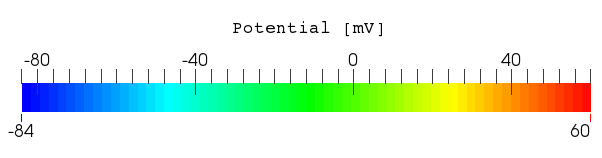
\includegraphics[height = 1.5 cm]{fig/numerical_example_mde+min_exp1_colourbar}
	} \\
\subfigure[3 ms]{
	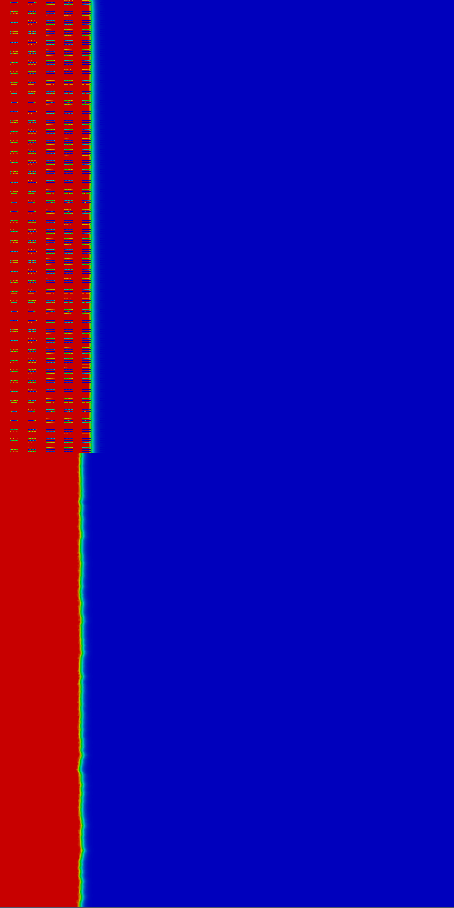
\includegraphics[height = 7 cm]{fig/Numerical_Experiments/ex3/numerical_example_mde+min_exp2_3ms}
	}	
\subfigure[17 ms]{
	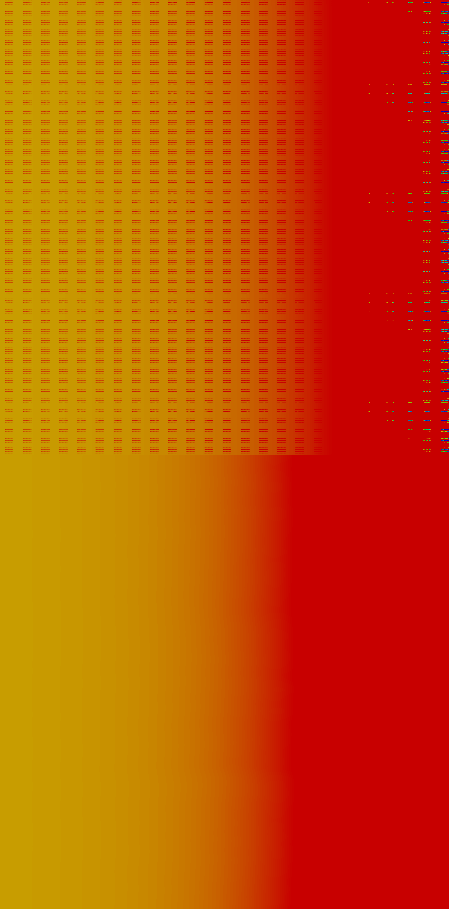
\includegraphics[height = 7 cm]{fig/Numerical_Experiments/ex3/numerical_example_mde+min_exp2_17ms}
	}
\caption{Exact (up) and Homogenized (down) solutions.} \label{fig:results_exp2}
\end{figure}


\section{Experiment \# 2: Tissue with Randomly Generated Fibrosis}

The collagen laminations are usually randomly distributed. In this example we try to emulate that by setting $\theta_c  \sim \mathcal{N}(\mu_c, \sigma_c)$ and $\theta_f \sim \mathcal{N}(\mu_f, \sigma_f)$, where $\sigma_c$ and $\mu_c$ are the mean and the standard deviation of a normal distribution. In particular, we will use the paramters of the table \ref{tab:ex4_parametros_random}:

\begin{table}[H]
\centering
\caption{ parameters use to generate the random fibrotic tissue mesh.}
\label{tab:ex4_parametros_random}
\begin{tabular}{@{}cc@{}}
\toprule
Parameter  & Value \\ \midrule
$\mu_c$    & 0.3   \\
$\mu_f$    & 0.5   \\
$\sigma_c$ & 0.2   \\
$\sigma_f$ & 0.3   \\ \bottomrule
\end{tabular}
\end{table}

Note that the $\mathbb{E}(\theta_c)$ and $\mathbb{E}(\theta_f)$ represent a tissue with a moderated level of fibrosis. In the figure \ref{fig:ex3_random} a portion of a domain generated with the parameters of the table \ref{tab:ex4_parametros_random} parameters can be observed.

\begin{figure}[H]
\centering
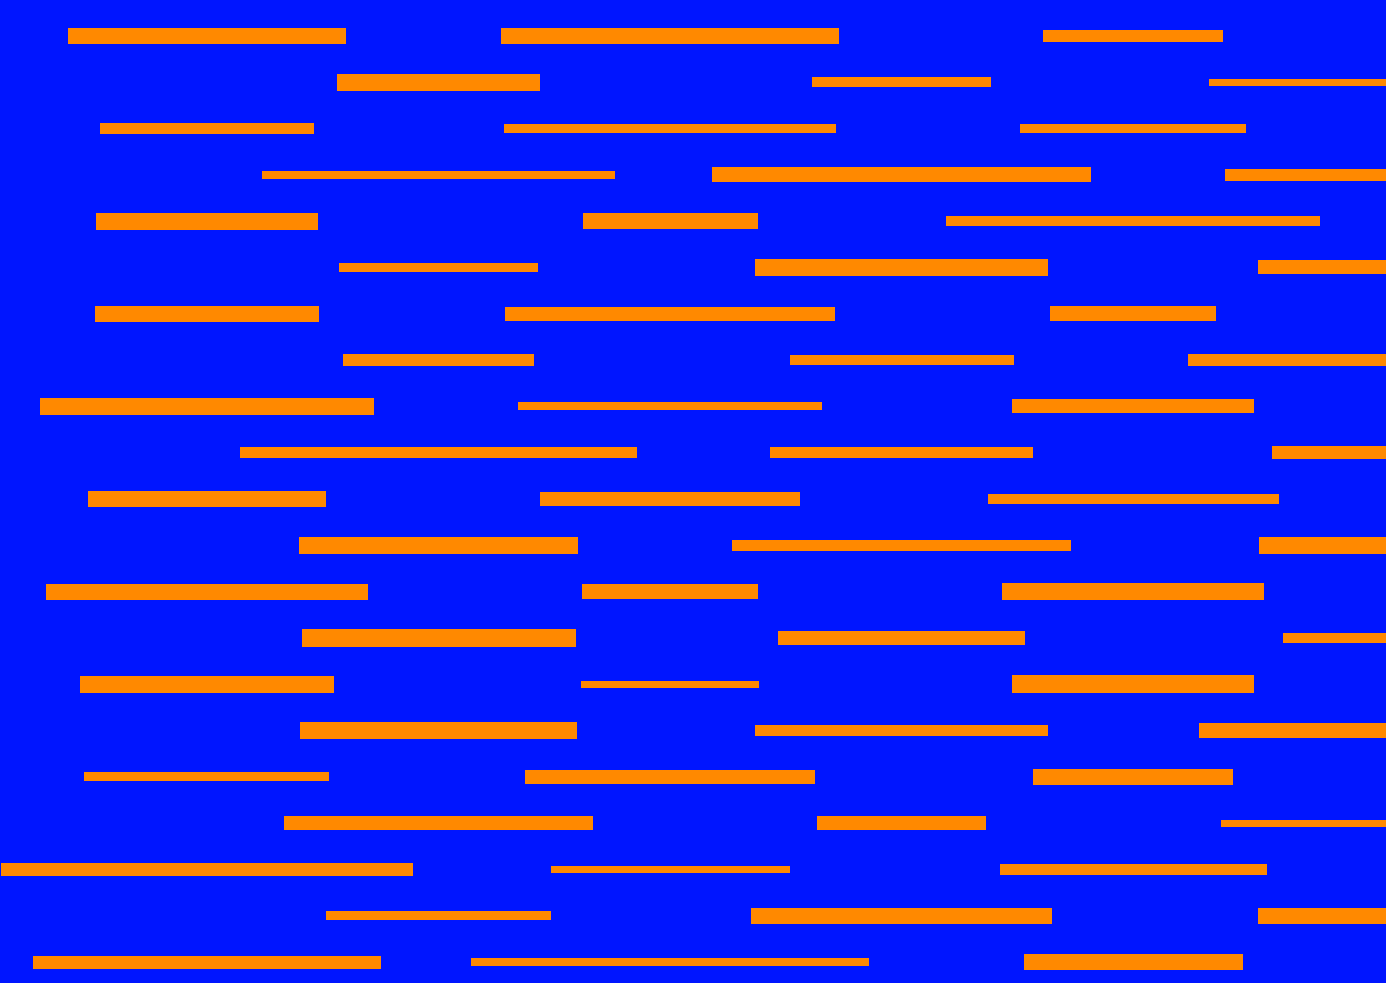
\includegraphics[height = 3.5 cm]{fig/Numerical_Experiments/ex4/random_mesh}
\caption{a zoom of a randomly generated mesh.} \label{fig:ex3_random}
\end{figure}


If the random values are not within a physiolocal range are recalculated. For $\theta_c$ we admit values from 0.15 (healthy tissue) to 0.45 (highly fibrotic tissue), and for $theta_f$ we admit values from 0.35 to 0.9. The choise of $\theta_f$ is done in order to get a tissue that emulates diffuse fibrosis, because values over 0.9 tends to generate collagen block-walls, i.e., stringy fibrosis.


\begin{figure}[H]
\centering
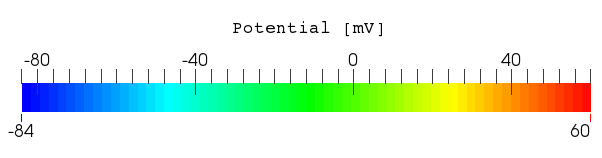
\includegraphics[height = 1.5 cm]{fig/numerical_example_mde+min_exp1_colourbar}
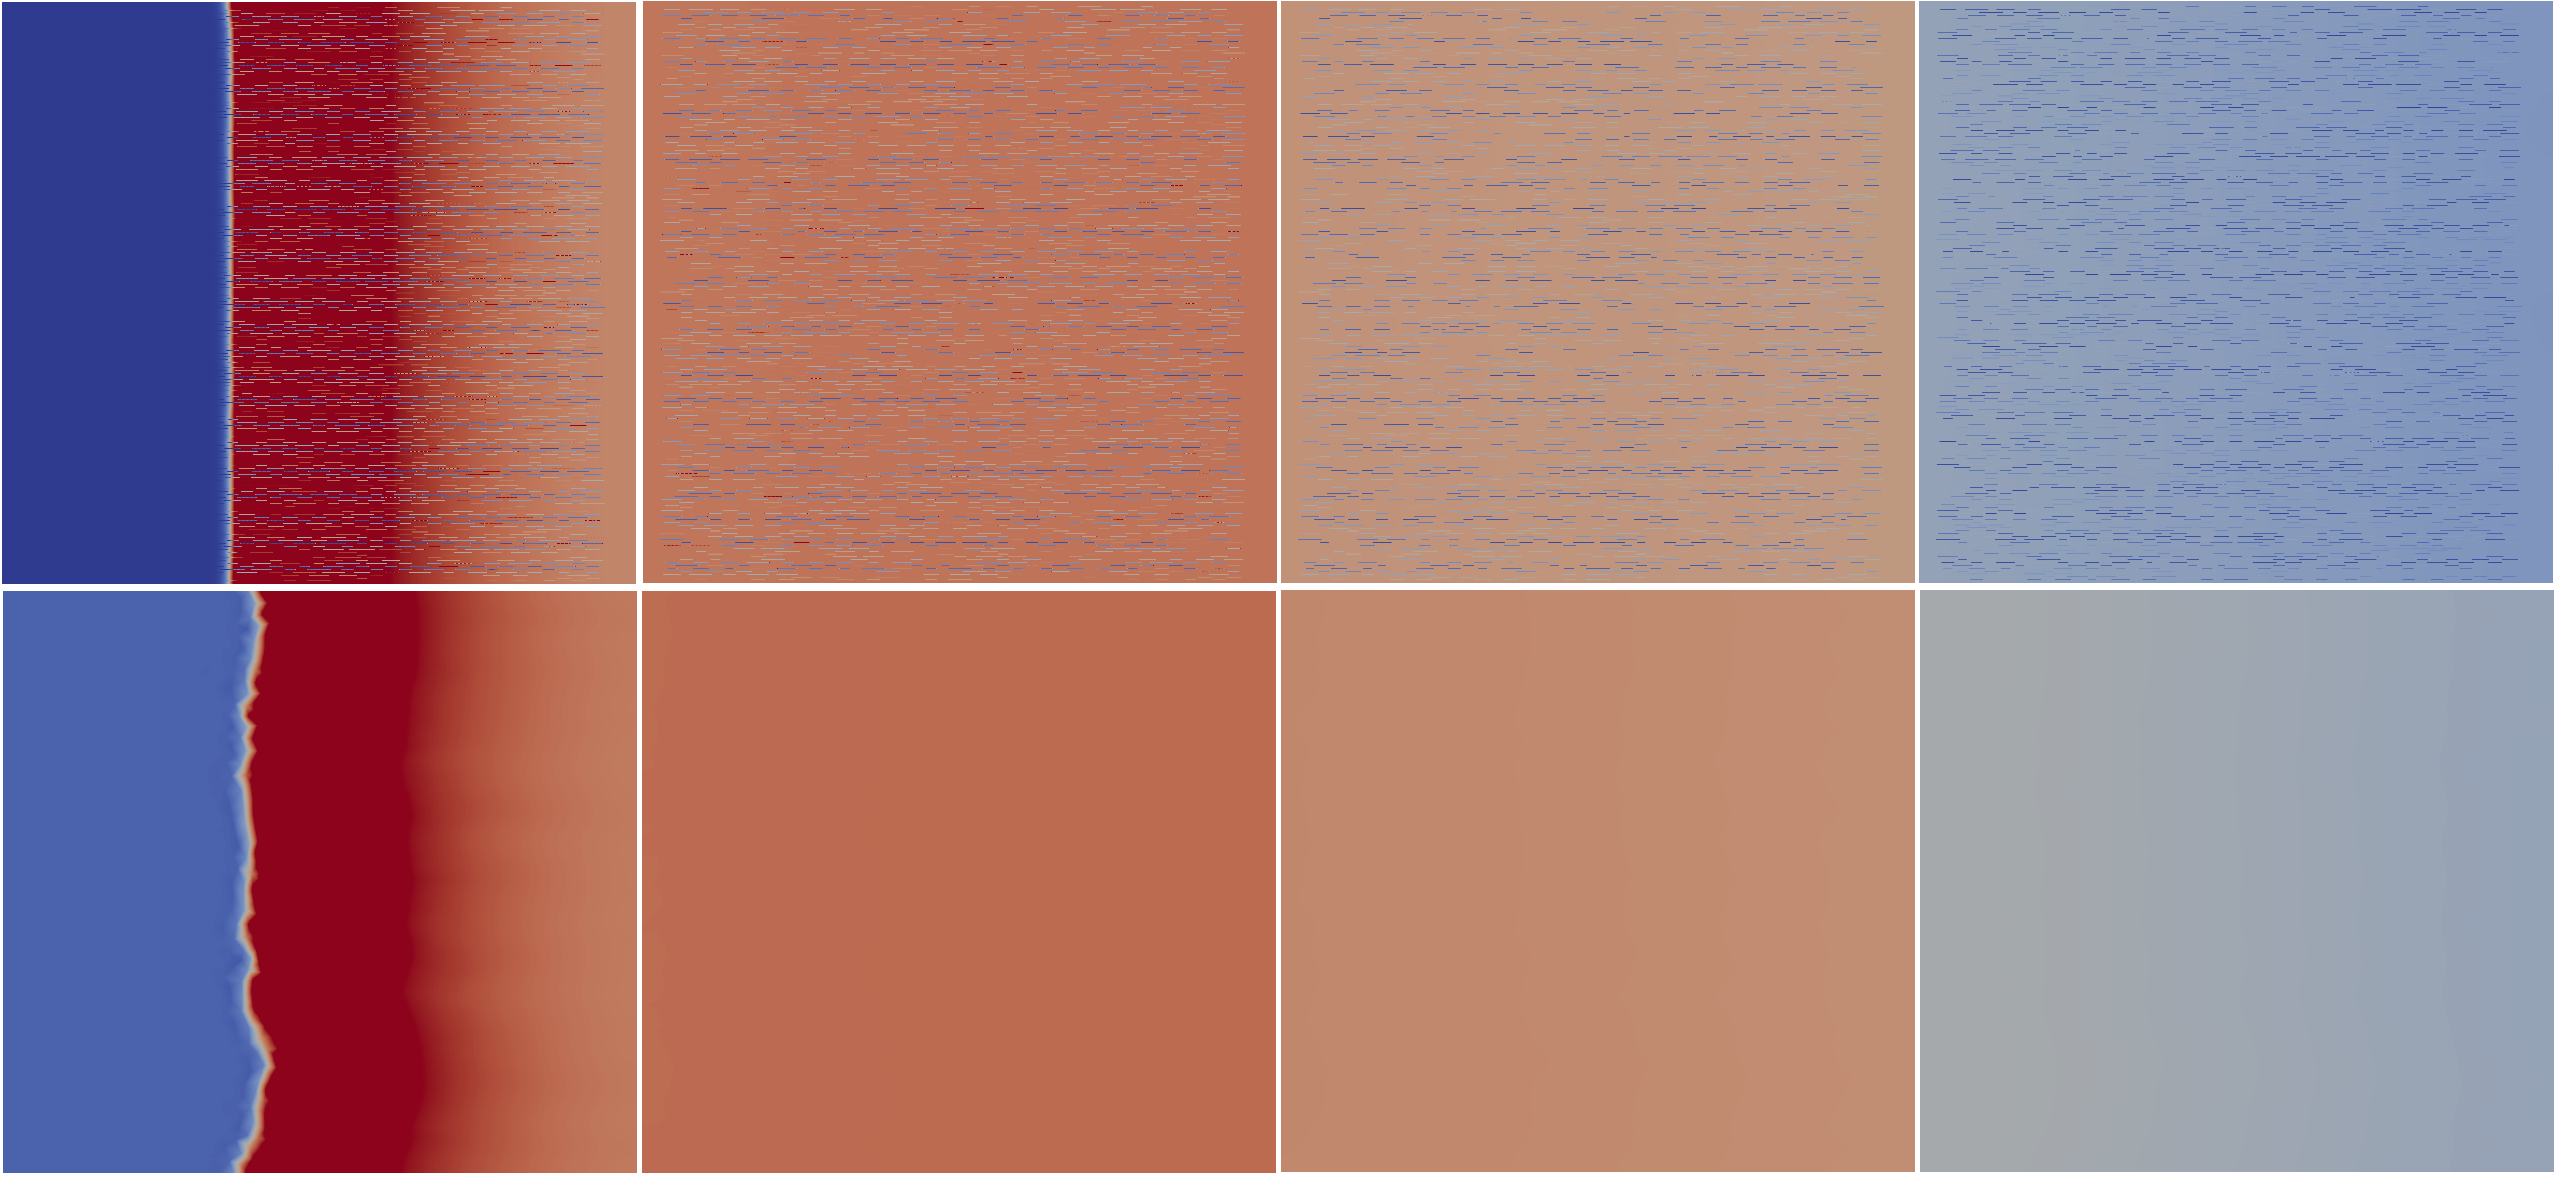
\includegraphics[height = 7 cm]{fig/Numerical_Experiments/ex4/results} 
\caption{ results of the experiment for $t = 30 ms$, $t = 50 ms$, $t = 150 ms$ and $t = 250 ms$ from left to right. The exact solution is shown at top, and the homogenized at the bottom. }
\end{figure}

The evolution of the error with time can be appreciated in table \ref{fig:ex4_error_L2}.

\begin{figure}[H]
\centering
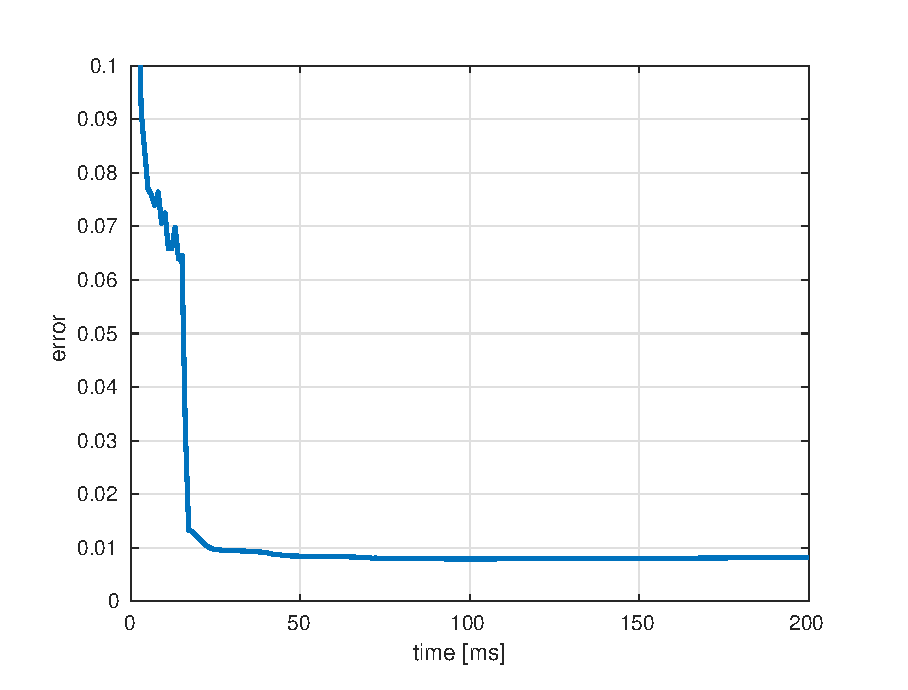
\includegraphics[height = 5 cm]{fig/Numerical_Experiments/ex4/error_L2.eps}
\caption{temporal evolution of the error.}
\label{fig:ex4_error_L2}
\end{figure}

The results are pretty similar to the non-random case. 
 
\end{document}
